%\documentclass[a0b,preview,portrait]{a0poster}
\documentclass[a0b,portrait,preview]{a0poster}
% With the word preview in the square bracket, your poster will be a4
% size, handy for previewing or submit to x4u queue for A0. 
% with preview removed, you get a file the right size for the HP
% large-format printer. This is a bit bigger than A0, the width is 
% exactly one imperial yard.

% This is so we can have multiple columns of text side-by-side
\usepackage{multicol,wrapfig}
\usepackage{xcolor}
%\usepackage{hyperref}
% This is the sideways spacing between the columns of  text
\columnsep=100pt 

% This is the thickness of the black line between the columns of text
\columnseprule=2pt
% This is the color of the columns
%My shaded gray
\definecolor{light-gray}{gray}{0.8} %0.95 is more similar to 1 (white), 0 would be black, 0.5 is in between
\def\columnseprulecolor{\color{light-gray}}

% this package gives you coloured text and various other simple
% graphics hacks. 
% Details in /usr/local/teTeX/texmf/doc/generic/pstricks/*
\usepackage{pstricks}
\usepackage[english]{babel}
\hyphenation{candidate re-so-nan-ces si-gni-fi-cant using si-mu-la-te sy-ste-ma-tic be-ne-fit}
%\psset{unit=1cm}

% Gives you the times font
\usepackage{times}

% Alllows you to include postscript files. Instructions in 
% /usr/local/teTeX/texmf/doc/latex/graphics/epslatex.ps 
\usepackage{graphicx}
\usepackage[utf8x]{inputenc} %This is necessary to handle accents

% Define names for some colours 
\newcmykcolor{Inblue}{1.00 0.37 0.00 0.00}
\newcmykcolor{Inred}{0.00 1.00 0.63 0.00}
\newcmykcolor{Inpurple}{0.50 1.00 0.40 0.00}
\newrgbcolor{Inmaroon}{0.4 0.0 0.4}
\newrgbcolor{darkblue}{0.0 0.0 0.5}
\newrgbcolor{darkgreen}{0.0 0.5 0.0}


% Colour used for figure captions. Change to suit your own preference
\newrgbcolor{captcolor}{0.0 .5 0.0}
\def\Journal#1#2#3#4{{#1}{\bf #2}(#4) #3}

\def\PMJ{ Proc.\ Phys.\ Math.\ Soc.\ Jap.}
\def\NCA{ Nuovo Cimento}
\def\NIM{ Nucl.\ Instrum.\ Methods}
\def\NIMA{{ Nucl.\ Instrum.\ Methods} \bf A}
\def\NPB{{ Nucl.\ Phys.} \bf B}
\def\NPP{{ Nucl.\ Phys.}}
\def\PLB{{ Phys.\ Lett.}  \bf B}
\def\PLL{{ Phys.\ Lett.}}
\def\PRL{ Phys.\ Rev.\ Lett.}
\def\PRD{{ Phys.\ Rev.} \bf D}
\def\ZPC{{ Z.\ Phys.} \bf C}
\def\EUR{{ Eur.\ Phys.\ J.} \bf C}
\def\CPC{{Comput.\ Phys.\ Commun.}}
\def\MODA{{Mod.\ Phys.\ Lett.} \bf A}
\def\REVM{{Rev.\ Mod.\ Phys.}}


\begin{document}


%  *** Begin code to draw blue border round poster ***
\psset{linewidth=0.5cm}
% Sets up lengths for frame
\newlength{\frameleft}
\newlength{\frameright}
\newlength{\frametop}
\newlength{\framebottom}
\setlength{\frameleft}{-2cm}
\setlength{\frameright}{\textwidth}
\addtolength{\frameright}{-\frameleft}
\setlength{\frametop}{2cm}
\setlength{\framebottom}{-\textheight}
\addtolength{\framebottom}{-\frametop}
% Draws a blue frame
%\psframe[linecolor=darkblue,cornersize=absolute,linearc=2]
%(\frameleft,\framebottom)(\frameright,\frametop)% need to overlay EOSMLS
%   *** Border finished *** 

% This is black magic to put a title at the top of the page.
% Thanks to Mark ``the magician'' Filipiak, although I have re-done a
% lot of the code here -- hopefully it is more robust.

% Make a box 0.55* width of poster for title and names
% If your title is long, replace 0.55 with something bigger and 
% make the box for the address smaller by the same amount.

%PUTTING LOGOS ON LEFT AND RIGHT SIDES OF THE PAGE
\begin{tabular}{p{0.13\linewidth} p{0.65\linewidth} p{0.2\linewidth}}
    
\includegraphics[height=7cm]{figure/iihe-logo.jpg} &
    \begin{center} 
    \vspace{-6cm} \veryHuge \bf Search for new physics at the LHC:\\ bump hunting in the dilepton spectra \\
\end{center} &
    
\includegraphics[height=7cm]{figure/ulb-logonorm.jpg}
        
\includegraphics[height=7cm]{figure/VUB_logo_compact.jpg}
\end{tabular}

\begin{minipage}[b]{0.99\linewidth} 
\begin{center}
%{\veryHuge \bf 
\vspace{1cm}
\large{Presented at the Colloquium ``Particle physics after the 2013 Nobel Prize'', organised by the Royal Academies for Sciences and the Arts of Belgium} \\
\huge \bf {\darkblue G.~Fasanella, A.~Randle-Conde, W. Fang and B.~Clerbaux for the CMS Collaboration} \\[0.7cm]

{\Large \rm \it
 Interuniversity Institute for High Energies (IIHE) - Université Libre de Bruxelles (ULB) and Vrije Universiteit Brussel (VUB), \\ 
 Boulevard du Triomphe, B-1050 Brussels, Belgium } 
 %Email contact: giuseppe.fasanella@ulb.ac.be ; arandlec@ulb.ac.be} \\[0.7cm]
% {\Large \rm \bf Belgian Physical Society - 21 May 2008, ULB, Brussels}

\end{center}
\vspace{0.5cm}

\begin{abstract} \darkblue
%\large
{
Resonances in the dielectron and dimuon decay channels arise in many well established theories beyond the standard model, like grand unified theories (GUT) or models 
proposing extra spatial dimension(s). The legacy results obtained from the LHC RUN1, using the full dataset collected by the CMS experiment in 2012 from proton-proton collisions 
at a center-of-mass energy of 8 TeV, and corresponding to an integrated luminosity of 20.6 fb$^{-1}$ are presented. In absence of a significant deviation from the standard model predictions, 
95\% confidence level limits are calculated.
Future prospect on RUN2 (data to be taken in years 2015-17) and RUN3 (years 2020-22) at a proton-proton center-of-mass energy of 13 or 14 TeV will be also presented.
}

\end{abstract}
\end{minipage}

\vspace{1cm}

% This is how many columns your poster will be broken into.
%                 |
%                 V
\begin{multicols}{3}

% This is the width your figures will be scaled to. Change this if you 
% change the number of columns.
\newlength{\figwidth}
\setlength{\figwidth}{25cm}

% Set to half of figwidth. Used for putting two figs side by side
\newlength{\fighalfwidth}
\setlength{\fighalfwidth}{10cm}

% Can't use the figure environment within multicolumns. Set up our own 
% counter for figures.
\newcounter{figscount}


%----------------------------------------------------------------------
%----------------------------------------------------------------------
%----------------------------------------------------------------------
{\red \section{\bf Search for New Heavy Neutral Bosons @ LHC RUN1}}
Many scenarios beyond the Standard Model (e.g. Grand Unification Theories~[1], extra spatial dimensions~[2]) involve new neutral bosons with masses in the TeV range.
If such heavy bosons exist they would manifest themselves as a narrow peak in the invariant mass spectrum that is dominated by the Drell-Yan (DY) process
($q\bar{q}\rightarrow l\bar{l}$) in these search channels.%({\darkgreen \figref{fig:dyprocessbis}}) 

 The legacy results obtained from the LHC RUN1, using the full dataset collected by the CMS experiment in 2012 from proton-proton collisions 
at a center-of-mass energy of 8 TeV, and corresponding to an integrated luminosity of 20.6 fb$^{-1}$ are presented~[3].

\begin{minipage}{\figwidth}
\vspace{1.0cm}
\unitlength=1cm
\begin{center}
{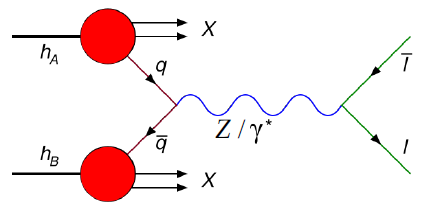
\includegraphics[width= 0.8\textwidth,height=10.0cm]{figure/dyprocessbis.png}}
\label{fig:dydiag}
\newline
\addtocounter{figscount}{1} 
{\small \captcolor Figure~\arabic{figscount}: Drell-Yan process diagram}
\end{center}
\vspace{1.5cm}
\end{minipage}

{\red \section*{\bf Event Selection}}
Events with two high energy electrons (muons) are selected, each of them with $E_t > 35$ GeV ($E_t > 45$ GeV).
Identification and isolation criteria are then applied to suppress backgrounds.
{\darkgreen Figure~2} shows the highest mass events passing the dedicated selections for the dielectron and the dimuon channels respectively.

\begin{minipage}{\figwidth}
\vspace{1.0cm}
\unitlength=1cm
\begin{center}
{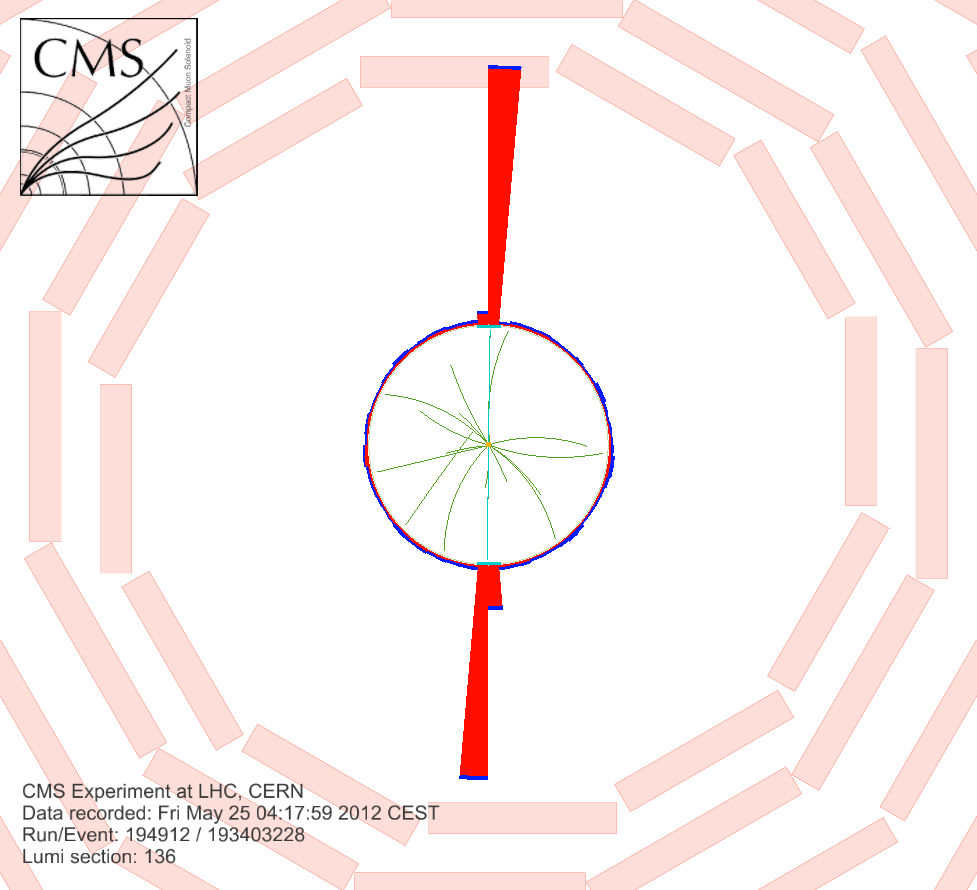
\includegraphics[width= 0.48\textwidth]{figure/ev1269GeV_rhophi.png}}
{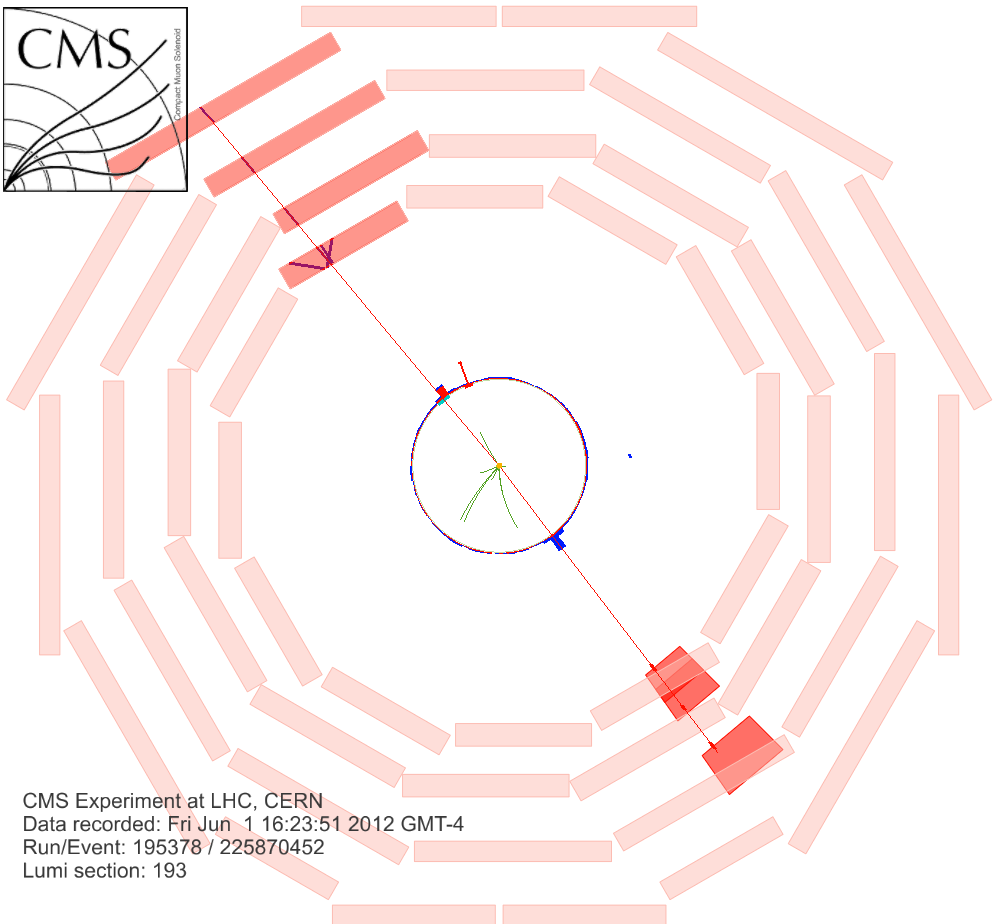
\includegraphics[width= 0.48\textwidth]{figure/ev_mumu_1418GeV_rhophi.png}}
%height=12.0cm
\newline
\addtocounter{figscount}{1} 
{\small \captcolor Figure~\arabic{figscount}: The highest mass event passing the dielectron selection (left) and the dimuon selection (right), having respectively an invariant mass of\\ 1269 GeV/$c^{2}$ and 1418 GeV/$c^{2}$}
\end{center}
\label{mass}
%\vspace{1.5cm}
\end{minipage}

\vspace*{1 cm}
%----------------------------------
{\red \section*{\bf Backgrounds}}
The \textbf{Drell--Yan process} is the most prominent (irreducible) background to the signal. 
However other processes (reducible backgrounds) have non negligible contribution: \textbf{multijet events from QCD processes} (where jets are misidentified as prompt leptons) and  
\textbf{top quark pair production events}, where the top quarks decay leptonically.
Data-driven methods have been designed to estimate the contamination of each of these processes.\\

{\red \section*{\bf Dilepton invariant mass spectra}}
The dilepton invariant mass spectra are shown in {\darkgreen figures~3~-~5}, where data are compared to the expected backgrounds.

\begin{minipage}{\figwidth}
\vspace{1.0cm}
\unitlength=1cm
\begin{center}
{\includegraphics[width= 0.8\textwidth]{figure/massHist19700pb}}%,height=12.0cm
\newline
\addtocounter{figscount}{1} 
{\small \captcolor Figure~\arabic{figscount}: Invariant mass spectrum of $ee$ events~[3]} %$e^{+}e^{-}$
\end{center}
\label{fig:limit}
\vspace{1.5cm}
\end{minipage}

{\darkgreen Figure~4} shows the dielectron channel split in the barrel-barrel and barrel-endcap regions of the ECAL calorimeter (as used for the limit calculation).

\begin{minipage}{\figwidth}
\vspace{1.0cm}
\unitlength=1cm
\begin{center}
{\includegraphics[width= 0.49\textwidth]{figure/massHist19700pbEBEB}}
{\includegraphics[width= 0.49\textwidth]{figure/massHist19700pbEBEE}}
%height=12.0cm
\newline
\addtocounter{figscount}{1} 
{\small \captcolor Figure~\arabic{figscount}: Invariant mass spectrum of $ee$ events split in barrel-barrel (left) and barrel-endcap (right) regions of the ECAL calorimeter~[3]}%$e^{+}e^{-}$
\end{center}
\label{mass}
%\vspace{1.5cm}
\end{minipage}

\begin{minipage}{\figwidth}
%\vspace{1.0cm}
\unitlength=1cm
\begin{center}
{\includegraphics[width= 0.7\textwidth]{figure/massHist20600pbMuon}}%,height=12.0cm
\newline
\addtocounter{figscount}{1} 
{\small \captcolor Figure~\arabic{figscount}: Invariant mass spectrum of $\mu\mu$ events~[3] }
\end{center}
\label{fig:limit}
\vspace{1.5cm}
\end{minipage}

%----------------------------------
{\red \section*{\bf Statistical analysis and results}}
The observed invariant mass spectra agree with expectations based on standard model processes.
\textbf{Since no new physics is observed, limits are set} on the possible contributions from narrow heavy resonances.
The variable under study is the ratio of the production cross section times branching ratio to two leptons for new heavy boson of spin 1 and the Z boson.
This cancels several sources of systematic uncertainty, including the one related to the integrated luminosity.

\begin{minipage}{\figwidth}
\vspace{1.2cm}
\unitlength=1cm
\begin{center}
{\includegraphics[width= 0.7\textwidth]{figure/zprime_MUMU_rereco_2012_nnlo_sf_v2}}
%height=12.0cm
\newline
\addtocounter{figscount}{1} 
{\small \captcolor Figure~\arabic{figscount}: Upper limits as a function of the resonance mass. The limits are shown for the dimuon final state~[3]}
%on the ratio of the production cross section times branching ratio to two muons}
\end{center}
\label{mass}
%\vspace{1.2cm}
\end{minipage}

\begin{minipage}{\figwidth}
\vspace{1.0cm}
\unitlength=1cm
\begin{center}
{\includegraphics[width= 0.7\textwidth]{figure/zprime_EE_rereco_2012_nnlo_sf_v2}}
%{\includegraphics[width= 0.49\textwidth]{figure/Figure_005-c}}
%height=12.0cm
\newline
\addtocounter{figscount}{1} 
{\small \captcolor Figure~\arabic{figscount}: Upper limits as a function of the resonance mass. The limits are shown for the dielectron final state~[3]}
%, for barrel-barrel channel (left) and
%barrel-endcap channel (right)}
%on the ratio of the production cross section times branching ratio to two electrons a}
\end{center}
\label{mass}
%\vspace{1.5cm}
\end{minipage}

\begin{minipage}{\figwidth}
\vspace{1.0cm}
\unitlength=1cm
\begin{center}
{\includegraphics[width= 0.7\textwidth]{figure/zprime_Combined_rereco_2012_nnlo_sf_v2}}
%%height=12.0cm
\newline
\addtocounter{figscount}{1} 
{\small \captcolor Figure~\arabic{figscount}: 
Upper limits as a function of the resonance mass. The limits are shown for the combined dielectron and dimuon channels~[3]}
%on the ratio of the production cross section times branching ratio to two leptons }
\end{center}
\label{mass}
\vspace{1cm}
\end{minipage}

\textbf{Lower limits on the resonance mass are derived}: a sequential standard model $Z'_{SSM}$ (heavy Z replica, with SM couplings to fermions) and a superstring-inspired $Z'_\psi$ lighter than 2960 GeV and 
2600 GeV respectively can be excluded at 95\% confidence level. These are the \textbf{most restrictive limits to date.}

\vspace{1,5cm}

%----------------------------------
{\red \section{\bf Future prospects @ LHC RUN2}}
\vspace*{0.cm}
{\darkgreen Figure~9} shows that the new data-taking at high energy is expected to benefit from a significant increase in the cross section for the production of heavy resonances. For example,
for a resonance of mass $\approx$ 2.5 TeV (from $q\bar{q}$ production mode) there is a factor $\approx$ 10 between the 13 TeV scenario and the 8 TeV scenario (end of RUN1)~[4].
This can make the discovery of a new TeV scale particle possible with a few fb$^{-1}$ of integrated luminosity.

RUN2 will consist in two periods of data-taking, the first one in 2015-2017, and the second one in 2019-2021. The expected total integrated luminosity is $\approx$~ 300 fb$^{-1}$.
At the end of RUN2 (see {\darkgreen figures~10~-~11}), a $Z'_{SSM}$ could be discovered up to masses of 5 TeV~[5].

%----------------------------------
\begin{minipage}{\figwidth}
%\vspace{1.0cm}
\unitlength=1cm
\begin{center}
{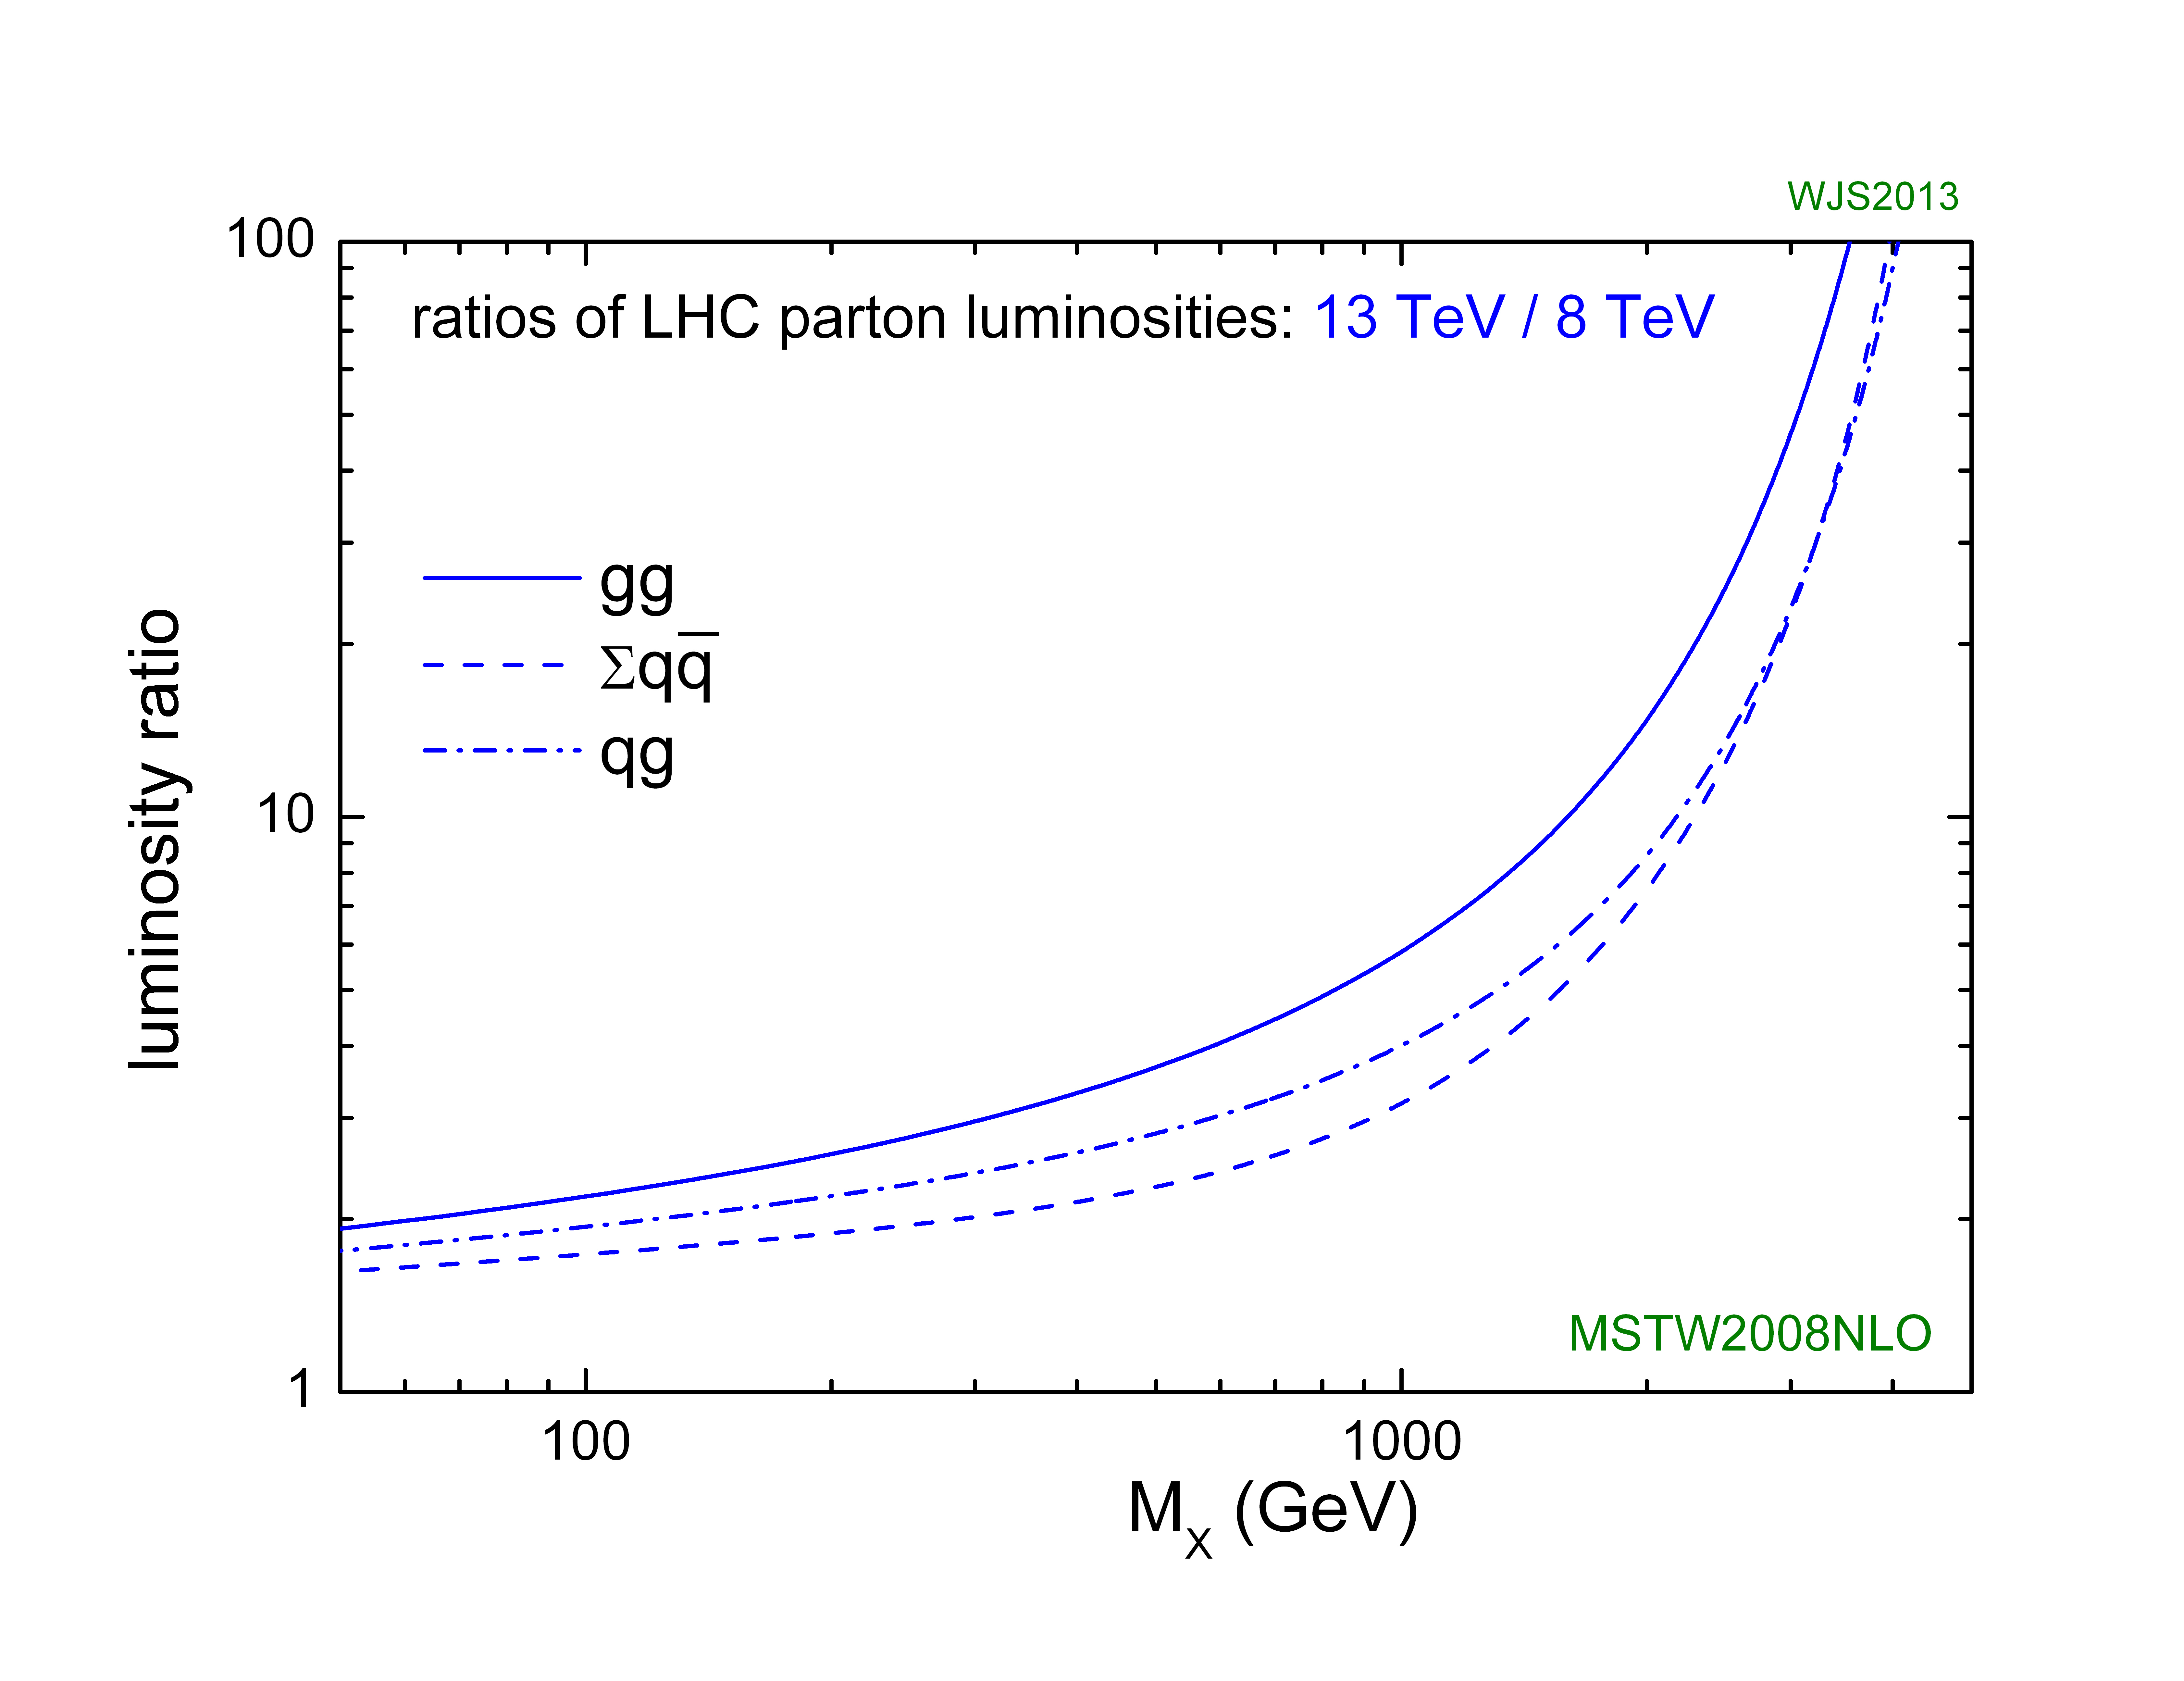
\includegraphics[width= 0.8\textwidth]{figure/lumi_scale.jpg}}%,height=12.0cm
\newline
\addtocounter{figscount}{1}
{\small \captcolor Figure~\arabic{figscount}: Ratio of LHC parton luminosities between 13 and 8 TeV~[4]} %5 $fb^{-1}$ @ 13 TeV vs 20 $fb^{-1}$ @ 8TeV}
\end{center}
\label{fig:limit}
\vspace{1.5cm}
\end{minipage}

%----------------------------------
{\red \section{\bf Discovery potential @ HL-LHC}}
In this section, the discovery potential for heavy neautral resonances ($Z'$) with the 14 TeV HL-LHC dataset (data-taking foreseen after 2023) at CMS is presented~[5].
The expected total integrated luminosity is $\approx$~ 3000 fb$^{-1}$.

In order to project the discovery potential of the RUN1 search to the HL-LHC scenarios, the background and signal yields are predicted using generator level simulation parameterized 
by the efficiencies and resolutions measured in the 8 TeV data.

Samples of $Z'$ events were also generated using PYTHIA and the interference between $Z'$ and Drell--Yan was not considered.
Signal and background events are simulated at generator level and smeared to simulate the detector response.
The dominant background for both dielectrons and dimuons channels is the Drell--Yan production of lepton pairs. 
The background due to $t\bar{t}$ production is found to self-veto above~1 TeV, because the boost of the top causes the lepton to fail isolation criteria due to the proximity of a b-jet.
The background due to WW production is expected to be the dominant non-DY background above 1 TeV, but is found to be small (1-2\% of the DY).

%----------------------------------
\begin{minipage}{\figwidth}
\vspace{1.0cm}
\unitlength=1cm
\begin{center}
{\includegraphics[width= 0.85\textwidth]{figure/zPrimeDiscovery300to3000fb}}%,height=12.0cm
\newline
\addtocounter{figscount}{1}
{\small \captcolor Figure~\arabic{figscount}: The minimum cross section times branching ratio for discovery as a function of dielectron mass for various luminosity scenarios~[5]}
\end{center}
\label{fig:limit}
%\vspace{1.5cm}
\end{minipage}

\begin{minipage}{\figwidth}
\vspace{1.0cm}
\unitlength=1cm
\begin{center}
{\includegraphics[width= 0.85\textwidth]{figure/zPrimeMuMuLimit}}%,height=12.0cm
\newline
\addtocounter{figscount}{1}
{\small \captcolor Figure~\arabic{figscount}: The minimum cross section times branching ratio for discovery as a function of dimuon mass for various luminosity scenarios~[5]}
\end{center}
\label{fig:limit}
\vspace{1.5cm}
\end{minipage}
%----------------------------------

The discovery potential reached in the dielectron and dimuon channels is shown in {\darkgreen figures~10-11}.
In both cases, the leading order cross section times branching ratio for various $Z'$ models is also shown.
At the end of the HL-LHC data-taking, a $Z'_{SSM}$ could be discovered up to masses of 6.2 TeV.

\vspace{1.5cm} %vertical space
{\darkblue 
References: \\
{\small
$[1]$ A. Leike, \textit{The Phenomenology of Extra Neutral Gauge Bosons}, Phys. Rept. 317 (1999) 143, \verb|[hep-ph/9805494]| \\%Z prime Psi
$[2]$ L. Randall, R. Sundrum, \textit{A Large Mass Hierarchy from a Small Extra Dimension}, Phys. Rev. Lett. 83 (1999) 3370, \verb|[hep-ph/9905221]| \\
$[3]$ The CMS Collaboration, \textit{Search for physics beyond the standard model in dilepton mass spectra in proton-proton collisions at $\sqrt{s}$ = 8 TeV}, CMS PAS EXO-12-061, \verb|[hep-ph/1412.6302]|, paper submitted to JHEP \\
$[4]$ Martin et al, \textit{Parton distributions for the LHC}, \verb|[hep-ph/0901.0002]|\\
$[5]$ The CMS Collaboration, \textit{Projected Performance of an Upgraded CMS Detector at the LHC and HL-LHC: Contribution to the Snowmass Process}, CMS Public Note CMS NOTE-2013/002 \\

}
}


\end{multicols}

\end{document}
